\documentclass[12pt]{report}
\usepackage[margin=1in]{geometry}
\usepackage{setspace}
\usepackage{xeCJK}
% \usepackage{ctex}
% \usepackage[sort]{natbib}
% \bibliographystyle{sb}
%     \bibpunct[:]{(}{)}{;}{a}{}{,}
\usepackage[colorlinks=false,hidelinks]{hyperref}  %change to true if you want to see links in color for drafting; hidelinks removes the boxes around links

\usepackage{doi} % turns dois into links

\usepackage{gb4e}\noautomath %% or use expex, as preferred

%%% Keep these 
\hypersetup{colorlinks=true,linkcolor=cyan,urlcolor=blue}
\usepackage{xcolor}
\usepackage{amsmath}
\usepackage{listings}
\definecolor{codegreen}{rgb}{0,0.6,0}
\definecolor{codegray}{rgb}{0.5,0.5,0.5}
\definecolor{codepurple}{rgb}{0.58,0,0.82}
\definecolor{backcolour}{rgb}{0.97,0.97,0.97}

%Code listing style named "python_style"
\lstdefinestyle{python_style}{
    backgroundcolor=\color{backcolour}, 
    commentstyle=\color{codegreen},
    keywordstyle=\color{magenta},
    numberstyle=\tiny\color{codegray},
    stringstyle=\color{codepurple},
    basicstyle=\linespread{.8}\ttfamily\footnotesize,
    breakatwhitespace=false,         
    breaklines=true,                 
    captionpos=b,                    
    keepspaces=true,                 
    numbers=left,                    
    numbersep=5pt,                  
    showspaces=false,                
    showstringspaces=false,
    showtabs=false,                  
    tabsize=2,
    language=python
}
\lstset{style=python_style}
\newcommand{\graylstinline}[1]{\colorbox{backcolour}{\lstinline{#1}}}

% \lstdefinestyle{inline_style}{
%     backgroundcolor=\color{backcolour}
% }
% \def\inline{\lstinline[basicstyle=inline_style]}

%%% Unicode font specifications
\usepackage[T1]{fontenc} % brings glyphs from 128 to 256, making accents easier
%\usepackage{textcomp} % more text symbols
\usepackage{fontspec,xltxtra,xunicode} % XeTeX font support stuff
% \usepackage{pifont}
\defaultfontfeatures{Mapping=tex-text}


%% FONTS
%\usepackage{libertine}
%\usepackage{times}

%\usepackage{comment} % permits a comment environment w/ varied versions

\usepackage{graphicx}


%%% Most of these are either optional or probably not needed for most people

\usepackage{anyfontsize}
%\usepackage{soul} % hyphenatable text formatting, basically
%\usepackage{wrapfig} % wrap around figures
% \usepackage{ragged2e}
\usepackage{booktabs} % enhances tables
\usepackage{colortbl}
% \usepackage{newtxmath,newtxtext}
% \usepackage{svg} % take this out if yale-crest isn't an svg
% \usepackage{epsfig}
\usepackage{titlesec} % more control over section and chapter headings


\DeclareGraphicsExtensions{.pdf,.png} %means you don't have to type the extension when including graphics; comment out if you prefer not to have this



% \setlength{\bibsep}{1.25pt} % sets bib spacing between items

\usepackage[normalem]{ulem}
%\usepackage{amssymb} % extra math symbols
%\usepackage[nointegrals]{wasysym}
% \usepackage{multirow} % multirow cells and tables
% \usepackage{mathrsfs} % supports rsfs font in math
%\usepackage{arydshln} % \hdashline and \cdashline
%\usepackage{pifont}
%\usepackage{stmaryrd} % compsci symbols, incl. \llbracket and \rrbracket
%\usepackage{mathtools}
% \usepackage{tikz} % drawing diagrams
%\usepackage{qtree} % tree drawing
%    \qtreecenterfalse

% \usepackage{tikz-qtree} % draw trees using TikZ using the syntax of Qtree
%\usepackage{framed} % \framed \shaded and \leftbar environments
% \usepackage[safe]{tipa} % ipa/phonetic characters % clashes with qtree if thety're both turned on
% \usetikzlibrary{decorations}
% \usetikzlibrary{decorations.pathreplacing}
% \usetikzlibrary{shapes,backgrounds}
 
\usepackage{url} % defines \url command
% \usepackage[all]{xy} % graphs and diagrams
% \usepackage{multicol} % multiple columns
% \usepackage{hanging}
 
\usepackage{parskip} % cleans up spacing layout for particular environments
    \parskip0.5ex

%\counterwithout{footnote}{chapter} 

\renewcommand{\contentsname}{目录} % redefines the heading of the ToC
\renewcommand{\listfigurename}{List of figures} % redefines the heading of the LoF
 
\renewcommand{\today}{\number\year 年 \number\month 月 \number\day 日}
% \usepackage[center]{titlesec}%chapter1修改为第1章
\titleformat{\chapter}{\raggedright\Huge\bfseries}{第\,\thechapter\,章}{1em}{}
\titleformat{\section}{\raggedright\Large\bfseries}{\,\thesection\,}{1em}{}
\titleformat{\subsection}{\raggedright\large\bfseries}{\,\thesubsection\,}{1em}{}
%\usepackage{enumerate} % old-ish way to enumerate
%\usepackage{enumitem} % better-ish way to enumerate
 

\usepackage{xcolor}
    \definecolor{dgreen}{rgb}{0.,0.6,0.}
    \definecolor{ochre}{cmyk}{0, .42, .83, .20}
    % \definecolor{forest}{cmyk}{.67, .23, .67, .18}
    % \definecolor{maroon}{cmyk}{0, 1, .07, .5}
    % \definecolor{peri}{cmyk}{.2,.2,0,0}
    % \definecolor{plum}{cmyk}{.48,.85,.29,.2}
    
%\gathertags % for forward references

\let\eachwordone=\sl
\singlegloss
\exewidth{(5.65)}
\addtolength{\footnotesep}{10pt}
% \addtolength{\bibsep}{4pt}

%% A bunch of cross-referencing shortcuts:
\newcommand{\sref}[1]{\S\ref{#1}}
\newcommand{\srefs}[2]{\S\S\ref{#1}--\ref{#2}}
\newcommand{\eref}[1]{(\thechapter.\ref{#1})}
\newcommand{\erefs}[2]{\eref{#1}--\eref{#2}}
\newcommand{\earef}[2]{(\ref{#1}\ref{#2})}
\newcommand{\sbref}[1]{(\S\ref{#1})}
\newcommand{\reff}[1]{\hspace*{\fill}{\mbox{#1}}}
% \newcommand{\refex}[2][]{\hfill\citep[#1]{#2}}
\newcommand{\reftex}[1]{\hspace*{\fill}\mbox{(#1)}}
\newcommand{\tref}[1]{Table~\ref{#1}\xspace}
\newcommand{\tpref}[1]{Table~\ref{#1} on page~\pageref{#1}\xspace}
\newcommand{\trefs}[2]{Tables~\ref{#1} and~\ref{#2}\xspace}
\newcommand{\fref}[1]{Figure~\ref{#1}\xspace}
\newcommand{\chref}[1]{Chapter~\ref{#1}\xspace}
\newcommand{\chrefs}[2]{Chapters~\ref{#1}--\ref{#2}\xspace}
\newcommand{\pref}[1]{page~\pageref{#1}\xspace}
\newcommand{\prefs}[2]{pages~\pageref{#1}--\pageref{#2}\xspace}
\newcommand{\aref}[1]{Appendix~\ref{#1}\xspace}

% \newcommand{\qcite}[1]{\citeauthor{#1}'s (\citeyear{#1})\xspace}

\newcommand{\comm}[1]{\textsl{\textbf{\large{{#1}}}}}
\newcommand{\tit}[1]{\textit{{#1}}}
\newcommand{\tbf}[1]{\textbf{{#1}}}
\newcommand{\tsc}[1]{\textsc{{#1}}}
\newcommand{\fno}[1]{\footnote{\small #1}}
\newcommand{\nfno}[1]{\footnote{\tbf{#1}}}
\newcommand{\ipa}[1]{\textipa{{#1}}}
\newcommand{\ul}[1]{\underline{{#1}}}
\renewcommand{\>}{\ensuremath >\xspace}
\newcommand{\<}{\ensuremath <\xspace}
\newcommand{\ortho}[1]{\ensuremath{<}#1\ensuremath{>}}
\newcommand{\uar}{\ensuremath\uparrow\xspace}

\newcommand{\var}{\ensuremath{\sim}\xspace}
\newcommand{\itipa}[1]{\textipa{\textsl{#1}}}

\newcommand{\tup}[1]{\textup{{#1}}}
\newcommand{\eg}{e.g.\@\xspace}
\newcommand{\ie}{i.e.\@\xspace}
\newcommand{\nd}{n.d.\@\xspace}
\newcommand{\cf}{cf.\@\xspace}


\begin{document}
\thispagestyle{empty}
\begin{titlepage}
    \begin{center}
        \vspace*{0pt}
        \makeatletter    
        \Large{\textbf{分布式机器学习}\\}
        \vspace{1ex}
        \Huge{\textbf{实验指导书}\\}
        \vspace{1ex}
        \small{课程号:85990072\\}
        \large
        \vspace{5ex}
        \textbf{授课教师:王智副教授}\\
        \vspace{.5ex}
        编者:袁新杰助教
        \vfill
        \large\textit{清华大学}\\
        \large\textit{清华大学深圳国际研究生院}\\
        \vspace{3ex}
        
\includegraphics[width=0.5\textwidth]{figures/tsinghua-icon.png}\\
        \vspace{2ex}
        \large
        % \textsc{Department of Linguistics}\\
        % \textsc{Yale University}\\
        \vspace{.5ex}
        % \normalsize DATE SUBMITTED\\
        \footnotesize \textcolor{gray}{[最后编辑于 \today]}
        \makeatother
    \end{center}
\end{titlepage}

\pagenumbering{roman}

% \addtocontents{toc}{\vspace{0pt}\protect\noindent\parbox[t]{\textwidth}{\normalsize\textcolor{black}{\textbf{Front matter}}}\par}

\clearpage
\phantomsection\addcontentsline{toc}{section}{前言}
\chapter*{前言}
\addtocounter{page}{-1}

可以介绍一下指导书结构,可以介绍一下我为什么想写这本指导书。感谢一下前任助教们

希望我这个是第一版,以后每年助教都可以持续更新迭代。

本指导书着重讲解环境配置与程序运行,对于具体分布式机器学习的算法实现,已由老师在课上讲解,实验指导书里不再赘述。【当然如果之后有人有兴趣把这部分补充上那就更好了】


助教 袁新杰 于2023年3月初

\stepcounter{page}


\singlespacing
\setstretch{0.95}
\tableofcontents
\addcontentsline{toc}{section}{目录}
\setstretch{1}

% \clearpage\chapter*{致谢}\addcontentsline{toc}{section}{致谢}




\normalsize
\newpage
\pagenumbering{arabic}
\doublespacing
\setlength{\parindent}{1.5em}

\chapter{环境配置与云计算资源使用}

本章将主要介绍分别使用本地计算资源、深研院计算资源和华为云计算资源时构建环境的方法。

\section{使用本地环境与GPU}\label{sec:local-env}

使用本地计算资源可以不收网络链接状况约束,随时随地调试程序,对于简单的项目,本地调试也可能更省时间。

本节以助教所使用的计算机为例,展示环境配置过程。助教使用的计算机系统与配置为:
\begin{itemize}
    \item 系统:windows10专业教育版;22H2
    \item 处理器:Intel(R) Core(TM) i7-8700 CPU 
    \item 内存:16GB
    \item 显卡:NVIDIA GeForce RTX 2060
    \item 编辑器:Visual Studio Code
\end{itemize}

\subsection{安装CUDA工具箱}
\textcolor{red}{TODO 这一部分只是贴了网址,没有写成教程}


对于包含英伟达显卡的计算机,我们推荐首先安装CUDA工具包以使用GPU加速计算。

\textcolor{red}{\emph{注意,仅包含英伟达GPU的计算机需要安装CUDA工具箱以使用GPU加速计算。使用核显或AMD显卡的计算机再后续步骤中使用CPU计算即可}}

GPU型号、CUDA工具包、PyTorch版本相互关联。因此需要一起规划好。

\url{https://developer.nvidia.com/zh-cn/cuda-gpus}
查看得到我的显卡的2060的算力为7.5,图\ref{fig:nvidia-rtx-2060-capability}。

\begin{figure}[htbp]
    \centering
    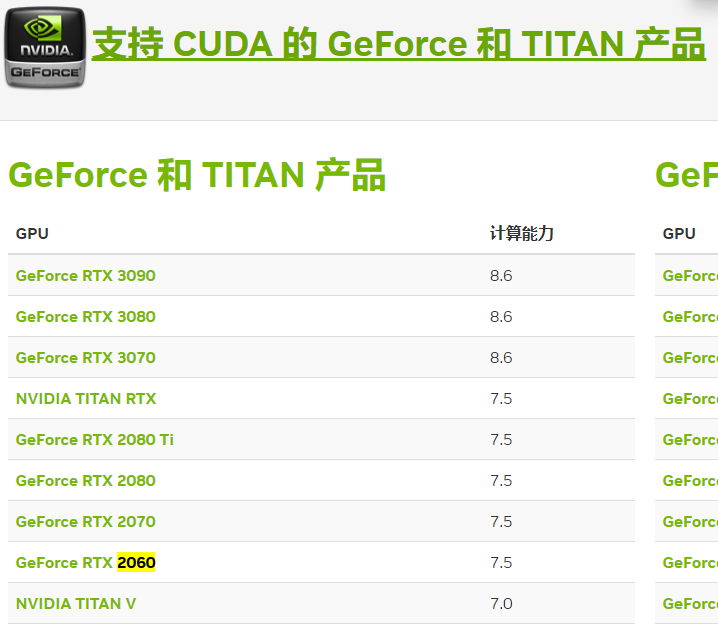
\includegraphics[width=0.7\textwidth]{figures/nvidia-rtx-2060-capability.png}
    \caption{fig:nvidia-rtx-2060-capability}
    \label{fig:nvidia-rtx-2060-capability}
\end{figure}


\url{https://en.wikipedia.org/wiki/CUDA}
查看得到支持我显卡的CUDA版本为$\geq$10.0,图\ref{fig:corresponding-cuda-version}。
\begin{figure}[htbp]
    \centering
    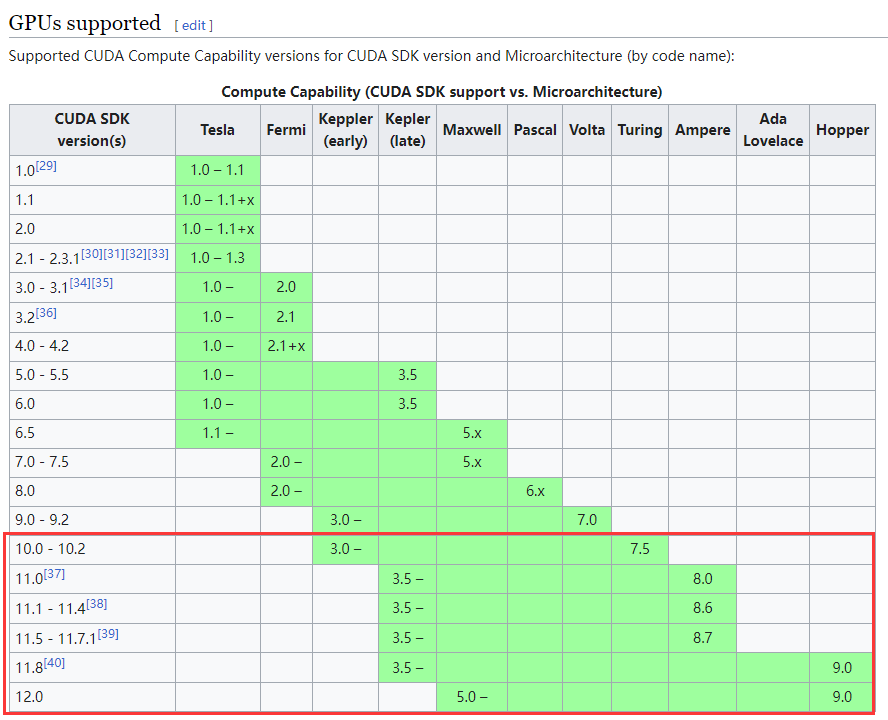
\includegraphics[width=0.7\textwidth]{figures/corresponding-cuda-version.png}
    \caption{fig:corresponding-cuda-version}
    \label{fig:corresponding-cuda-version}
\end{figure}

\url{https://docs.nvidia.com/cuda/cuda-toolkit-release-notes/index.html}
同时CUDA对显卡驱动的最低版本也提出了要求,但显卡驱动对CUDA向下兼容,因此一般安装了最近发布的显卡驱动版本即可,无需与CUDA版本特别对应。


\url{https://pytorch.org/get-started/locally/}
最后要注意,PyTorch并不一定支持最新的CUDA版本,因此安装前再去PyTorch上看一眼PyTorch支持哪些CUDA版本,图\ref{fig:cuda-version-constrained-by-pytorch}。
\begin{figure}[htbp]
    \centering
    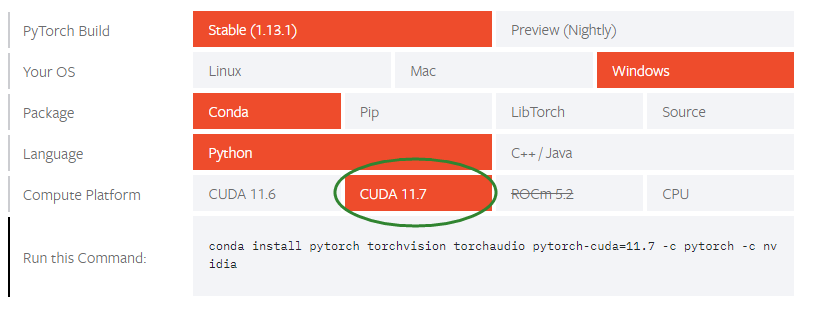
\includegraphics[width=0.7\textwidth]{figures/cuda-version-constrained-by-pytorch.png}
    \caption{fig:cuda-version-constrained-by-pytorch}
    \label{fig:cuda-version-constrained-by-pytorch}
\end{figure}

我们发现PyTorch最高支持到CUDA 11.7,满足显卡算力对CUDA版本$\geq$10.0的要求,因此我们可以选择安装CUDA 11.7。

选择对应版本CUDA安装包并下载安装, 安装过程略,图\ref{fig:select-cuda-version}。
\url{https://developer.nvidia.com/cuda-toolkit-archive}

\begin{figure}[htbp]
	\centering
	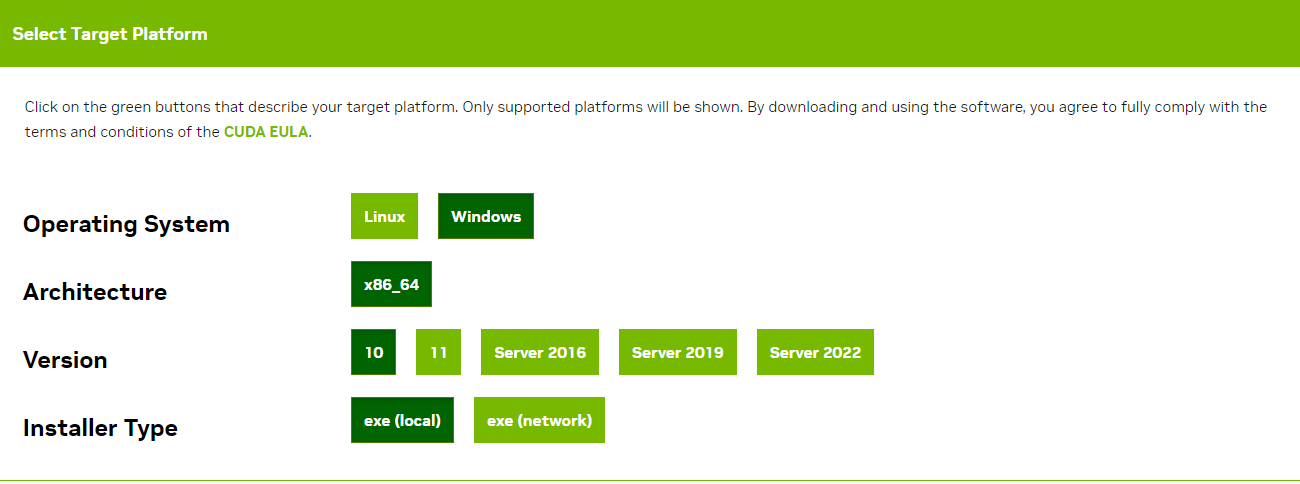
\includegraphics[width=0.7\textwidth]{figures/select-cuda-version.png}
	\caption{fig:select-cuda-version}
	\label{fig:select-cuda-version}
\end{figure}

在这一步完成后,我们打开终端输入\graylstinline{nvcc -V}以及\graylstinline{nvidia-smi}应当分别能看到图\ref{fig:nvcc-v-install-success}和图\ref{fig:nvidia-smi-install-success}类似的输出,这说明我们安装完成。

\begin{figure}[htbp]
	\centering
	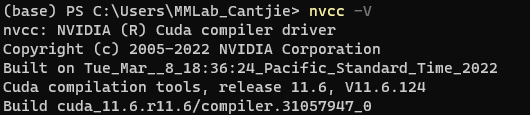
\includegraphics[width=0.7\textwidth]{figures/nvcc-v-install-success.png}
	\caption{caption:nvcc-v-install-success}
	\label{fig:nvcc-v-install-success}
\end{figure}

\begin{figure}[htbp]
	\centering
	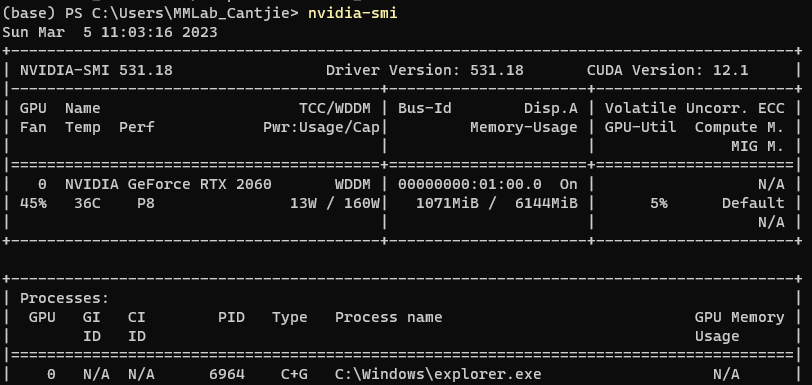
\includegraphics[width=0.7\textwidth]{figures/nvidia-smi-install-success.png}
	\caption{caption:nvidia-smi-install-success}
	\label{fig:nvidia-smi-install-success}
\end{figure}

\subsection{安装Anaconda}

我们可能同时有多个项目或作业在处理,而不同的项目或作业可能使用了不同python版本、不同的工具包等,为了避免冲突,我们通常会为每一个项目或作业指定一个虚拟环境,以使得各个环境之间互不干扰。为此,我们Anaconda以创建并管理虚拟环境。

安装过程参考官网文档即可:
\url{https://docs.anaconda.com/anaconda/install/windows/}

安装完成后启动终端,输入\graylstinline{conda -V},如正确显示conda版本则说明安装成功。
\begin{figure}[htbp]
	\centering
	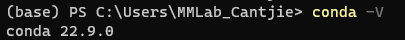
\includegraphics[width=0.7\textwidth]{figures/conda-install-success.png}
	\caption{CAPTION holder}
	\label{LABEL holder}
\end{figure}

\subsection{创建虚拟环境并安装PyTorch} \label{subsec:local-env-create}

安装完成conda后,我们新建一个预装了Python的、用来完成本门课程的虚拟环境。

需要注意的是,PyTorch和Python版本也需要对应,在\url{https://github.com/pytorch/vision#installation}中,我们发现torch 1.13要求python 介于3.7.2和3.10之间。

\begin{figure}[htbp]
	\centering
	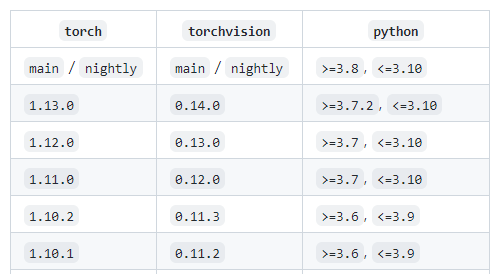
\includegraphics[width=0.7\textwidth]{figures/pytorch-python-version-compability.png}
	\caption{CAPTION holder}
	\label{LABEL holder}
\end{figure}

打开终端,输入下面命令以利用conda新建环境,
\begin{lstlisting}
    $ conda create --name <envname> python=3.9
\end{lstlisting}
将其中<envname>改成自定义的环境名称,如助教自己选择的distributedml。

新建完成后,通过\graylstinline{conda activate <envname>}进入环境。在pytorch官网安装页面\url{https://pytorch.org/get-started/locally/}选择对应的pytorch版本、系统版本等,复制给出的命令并运行。

\begin{figure}[htbp]
	\centering
	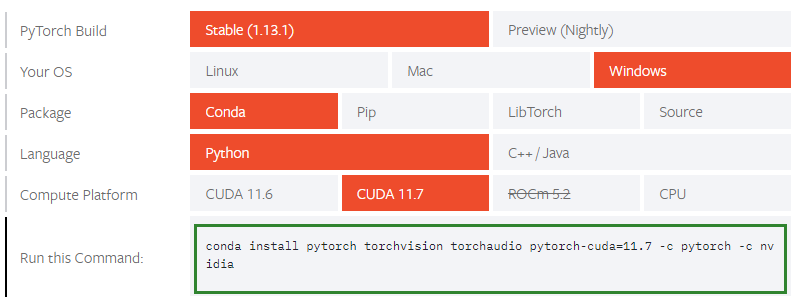
\includegraphics[width=0.7\textwidth]{figures/pytorch-install-command.png}
	\caption{CAPTION holder}
	\label{fig:pytorch-install-command}
\end{figure}

安装完成后,进入Python就可以\graylstinline{import torch}了,如图\ref{fig:pytorch-install-success}.

\begin{figure}[htbp]
	\centering
	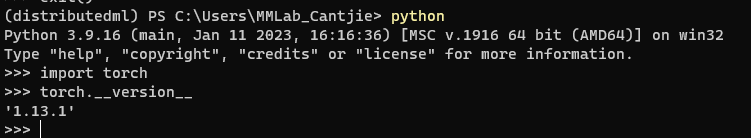
\includegraphics[width=0.7\textwidth]{figures/pytorch-install-success.png}
	\caption{caption:pytorch-install-success}
	\label{fig:pytorch-install-success}
\end{figure}

\subsection{安装其他包}

如果我们还想要安装其他包,比如同学们画图常用的matplotlib包,该怎么办呢?在\graylstinline{conda activate <envname>}进入环境后,直接通过\graylstinline{conda install matplotlib}就可以了。

% \subsection{使用VSCode编辑python文件}

% 以实验一为例,VSCode安装Python插件后,


\section{使用虚拟环境与本地GPU}

上面的本地环境配置不可为不复杂,CUDA、显卡型号、显卡驱动、PyTorch、Python等版本需要手动一一对应起来安装。那有没有什么更简单的利用本机GPU计算资源的方法呢?

在这一节,我们介绍直接利用Docker镜像搭配环境的方法。

\subsection{安装并配置Docker引擎}

首先在官网下载安装包\url{https://docs.docker.com/desktop/install/windows-install/},安装过程略。

在安装完成后启动Docker Desktop,在windows下,很可能会报错(具体内容是啥助教忘了截图了),一般错误的原因是缺少wsl2和hyper-v。

为了启用hyper-v,在控制面板中按照图\ref{fig:turn-on-hyper-v}中的操作选中Hyper-V并确定。
\begin{figure}[htbp]
	\centering
	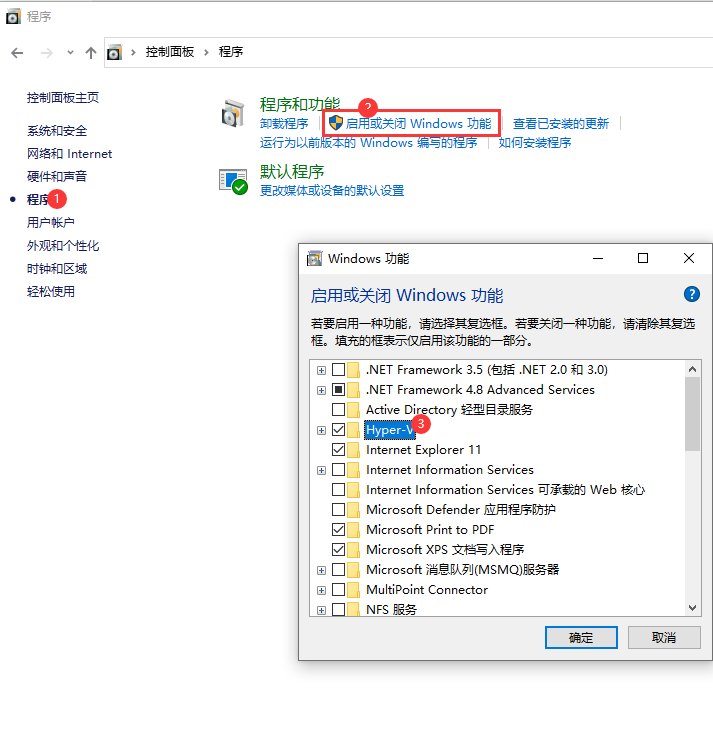
\includegraphics[width=0.7\textwidth]{figures/turn-on-hyper-v.png}
	\caption{caption:turn-on-hyper-v}
	\label{fig:turn-on-hyper-v}
\end{figure}

为了启用wsl2,参考\url{https://learn.microsoft.com/en-us/windows/wsl/install},在终端下输入\graylstinline{wsl --install}等待安装完成即可。

\begin{figure}[htbp]
	\centering
	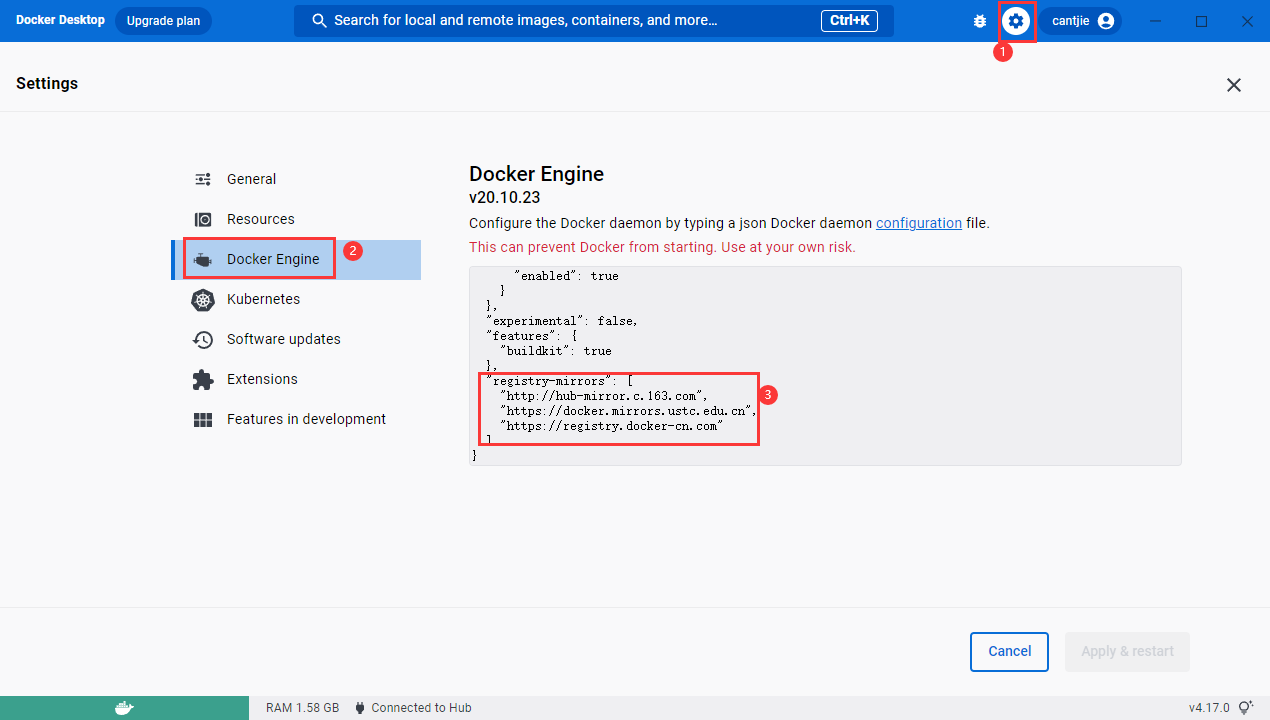
\includegraphics[width=0.7\textwidth]{figures/docker-mirrors-setting.png}
	\caption{caption:docker-mirrors-setting}
	\label{fig:docker-mirrors-setting}
\end{figure}

安装完成后启动Docker Desktop,为了加速下载,可以按照图\ref{fig:docker-mirrors-setting}所示方法为Docker指定国内镜像服务器,即在原本的配置中加入如下内容。
\begin{lstlisting}
    "registry-mirrors": [
        "http://hub-mirror.c.163.com",
        "https://docker.mirrors.ustc.edu.cn",
        "https://registry.docker-cn.com"
    ]
\end{lstlisting}

启动终端,输入\graylstinline{docker --version},如图\ref{fig:docker-install-success},正常返回Docker版本就说明安装成功了。
\begin{figure}[htbp]
	\centering
	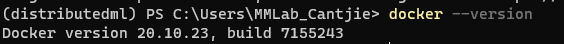
\includegraphics[width=0.7\textwidth]{figures/docker-install-success.png}
	\caption{caption:docker-install-success}
	\label{fig:docker-install-success}
\end{figure}


\subsection{搜索并下载PyTorch镜像}

Dockerhub是一个共享镜像的平台\url{https://hub.docker.com/}。所谓镜像,类似于一个操作系统的iso文件:我们拿到iso文件后可以创建使用该操作系统的虚拟机;而当我们拿到镜像后,也可以利用该镜像创造一个使用该镜像的容器,即容器是一个镜像的实例。

因此,如果有人在某个容器中把CUDA、PyTorch、Python等环境都配置好,并打包成镜像共享给我们,我们就可以免去复杂的安装过程,从而直接使用镜像生成容器,在容器中直接运行我们所写的脚本。

在DockerHub中,我们搜索\graylstinline{pytorch/pytorch},可以找到对应的这个镜像\url{https://hub.docker.com/r/pytorch/pytorch}。点击网页中的Tags标签页,我们可以从图\ref{fig:pytorch-image-tags-web}看到这个镜像就是已经把PyTorch和CUDA安装好了的,我们直接使用这个镜像就好啦!

\begin{figure}[htbp]
	\centering
	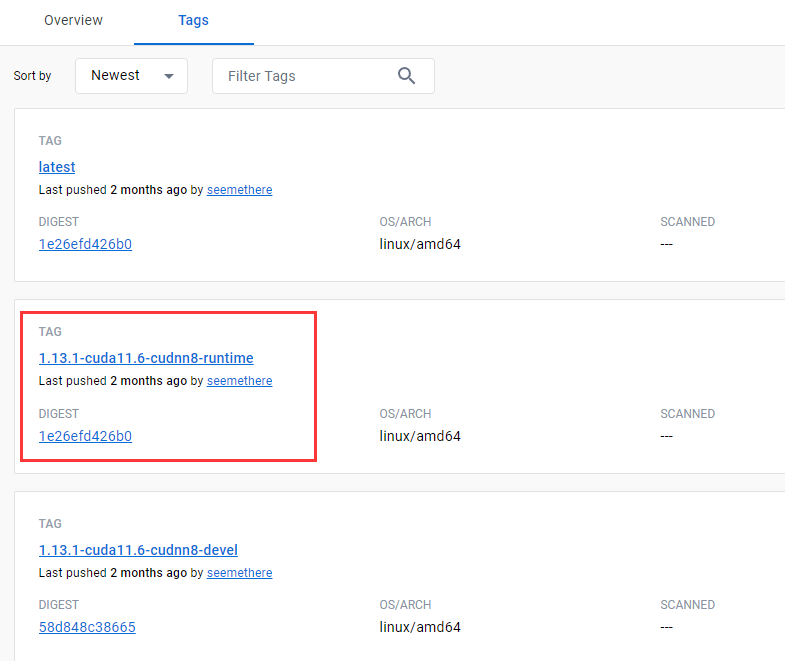
\includegraphics[width=0.7\textwidth]{figures/pytorch-image-tags-web.png}
	\caption{caption:pytorch-image-tags-web}
	\label{fig:pytorch-image-tags-web}
\end{figure}

下载这个镜像前,还需要登录的。首先去注册个账号,然后打开终端,输入\graylstinline{docker login}登录。

然后就可以通过这条命令下载这个镜像了:

\begin{lstlisting}
    $ docker pull pytorch/pytorch:1.13.1-cuda11.6-cudnn8-runtime
\end{lstlisting}


这个镜像比较大,下载需要一点时间。完成后,我们再输入\graylstinline{docker image list}就可以看到这个镜像了,见图\ref{fig:docker-image-list-pytorch}。
\begin{figure}[htbp]
	\centering
	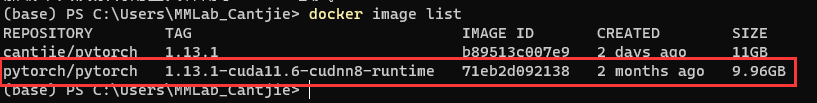
\includegraphics[width=0.7\textwidth]{figures/docker-image-list-pytorch.png}
	\caption{caption:docker-image-list-pytorch}
	\label{fig:docker-image-list-pytorch}
\end{figure}

\subsection{启动容器}

下载完镜像,我们该通过这个镜像启动一个容器了,我们需要到容器里看看这个容器里面是不是有我们需要的环境。

打开终端,输入
\begin{lstlisting}
    $ docker run -it pytorch/pytorch:1.13.1-cuda11.6-cudnn8-runtime
\end{lstlisting}
我们发现我们进入了一个linux系统,进去运行一下\graylstinline{nvidia-smi}试试,诶,怎么command not found,看不到显卡。这是因为容器启动时没有给他指定GPU。我们输入\graylstinline{exit},然后加上GPU参数再试一下
\begin{lstlisting}
    $ docker run --gpus all -it pytorch/pytorch:1.13.1-cuda11.6-cudnn8-runtime 
\end{lstlisting}

进入容器后,我们输入\graylstinline{nvidia-smi}等命令,查看运行结果,如图\ref{fig:docker-pytorch-container-env-check}所示,发现正是我们所需要的环境。
\begin{figure}[htbp]
	\centering
	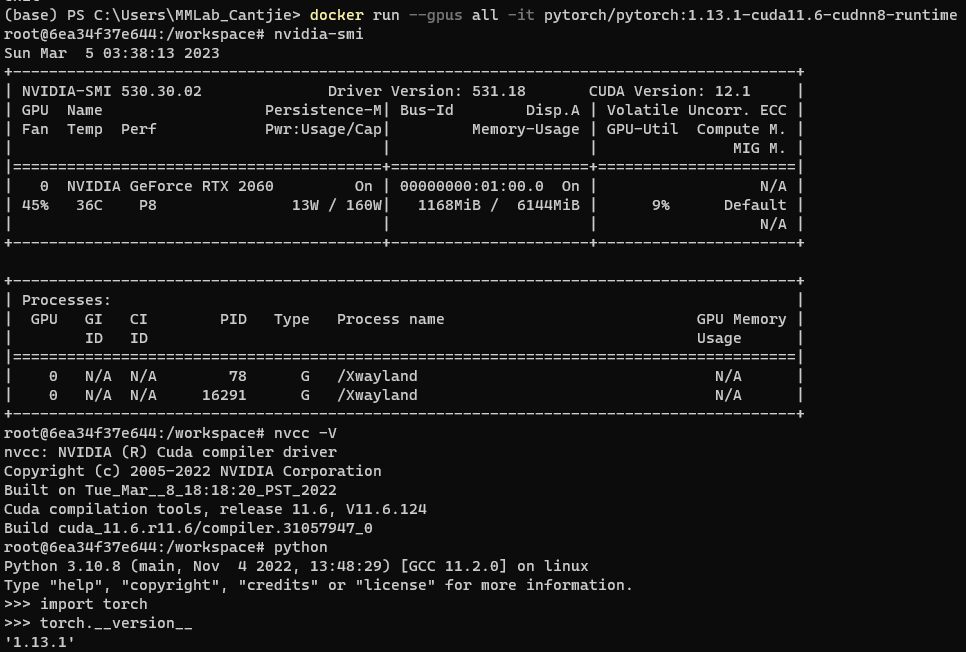
\includegraphics[width=0.7\textwidth]{figures/docker-pytorch-container-env-check.png}
	\caption{caption:docker-pytorch-container-env-check}
	\label{fig:docker-pytorch-container-env-check}
\end{figure}


\subsection{安装新包后重新打包成镜像}\label{subsec:container-to-image}

但是,也有一些包在默认的镜像里是没有的,万一我们需要这些包,比如matplotlib包,难道我们要每次启动新的容器之后都手动通过\graylstinline{conda install}安装一下么?不用的,我们安装一次之后,将这个容器重新打包成一个新的镜像就好了!我们之后再用,就用新的镜像了。

\begin{figure}[htbp]
	\centering
	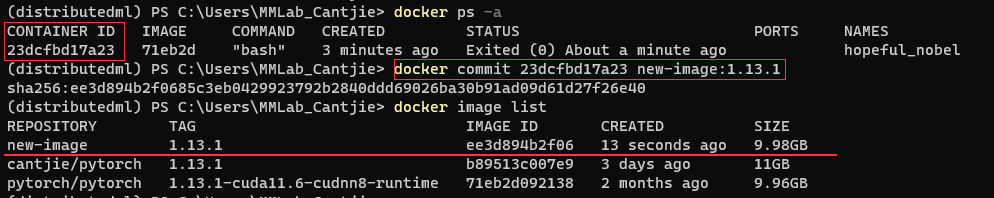
\includegraphics[width=1\textwidth]{figures/docker-commit-new-image.png}
	\caption{caption:docker-commit-new-image}
	\label{fig:docker-commit-new-image}
\end{figure}

在刚才启动的容器里,我们输入\graylstinline{conda install matplotlib},安装完成后,输入\graylstinline{exit}退出容器。回到windows下的命令行,输入\graylstinline{docker ps -a}查看所有容器,如图\ref{fig:docker-commit-new-image}所示,我们发现刚刚安装了matplotlib的容器的id为\graylstinline{23dcfbd17a23}。接下来,我们运行
\begin{lstlisting}
	$ # docker commit <containerID> <new-image-name>:<tags>
	$ docker commit 23dcfbd17a23 new-image:1.13.1
\end{lstlisting}
便将容器打包成了一个镜像。输入\graylstinline{docker image list},便可以看到我们新建的容器了。

以后就都可以用这个新镜像了,可是如何使用这个环境呢,我们留到完成具体实验内容的时候再来讲。

\subsection{限制Docker内存占用(可选)}

由于docker占用内存很大,对于内存不足的电脑可能造成卡顿现象,可以通过修改配置文件限制其内存占用。

修改C:\textbackslash users\textbackslash<username>\textbackslash .wslconfig 

\begin{lstlisting}
[wsl2]
memory=6GB
swap=6GB
swapfile=E:\\wsl-swap.vhdx
\end{lstlisting}



\section{使用华为云计算资源}\label{sec:huawei-cloud-usage}
\textcolor{red}{TODO 申请完计算资源之后完成这部分教程}


\section{使用深研院计算资源}

\textcolor{red}{\emph{注意,在该平台启动的开发环境需要首先手动调整一下DNS服务器,即在\graylstinline{/etc/resolv.conf}最上方添加一行“\graylstinline{nameserver 114.114.114.114}”即可。}}

助教会为同学们下发用户名和密码。使用自己的账户信息登录网址:\url{http://10.103.9.27:30000/}(或使用助教的域名\url{http://sigs-gpu.cantjie.com:30000})

\subsection{创建开发环境}

登录系统后,我们需要创建一个开发环境。如图\ref{fig:sigs-platform-dev-env-before-create}所示,首先在左侧边栏选择AI分区->开发环境,然后点击创建。

\begin{figure}[htbp]
	\centering
	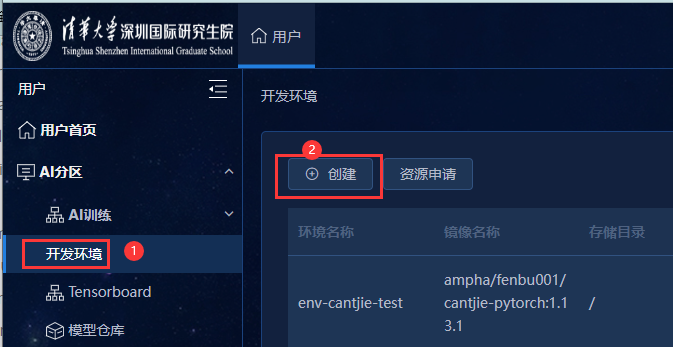
\includegraphics[width=0.7\textwidth]{figures/sigs-platform-dev-env-before-create.png}
	\caption{caption:sigs-platform-dev-env-before-create}
	\label{fig:sigs-platform-dev-env-before-create}
\end{figure}

在弹出的窗口图\ref{fig:sigs-platform-dev-env-create}中,设置环境名称、镜像、储存位置、资源规格等信息。其中,当与小组同学共享账号时,请不要直接选择默认的资源规格,请通过自定义,限制环境所需的CPU核心数量、储存空间大小和显卡数量。对于我们的实验,系统自带的镜像已基本可以满足需求,因此在镜像选择中,按图\ref{fig:sigs-platform-dev-env-image-selection}所示选择superadmin/pytorch:1.12.0-cuda11.3-cudnn8-runtime-2即可(注意末尾的-2,带-2的版本为本学期初根据课程需求定制的版本,不带-2的版本使用ssh连接进入后会找不到合适环境。)。

\begin{figure}[htbp]
	\centering
	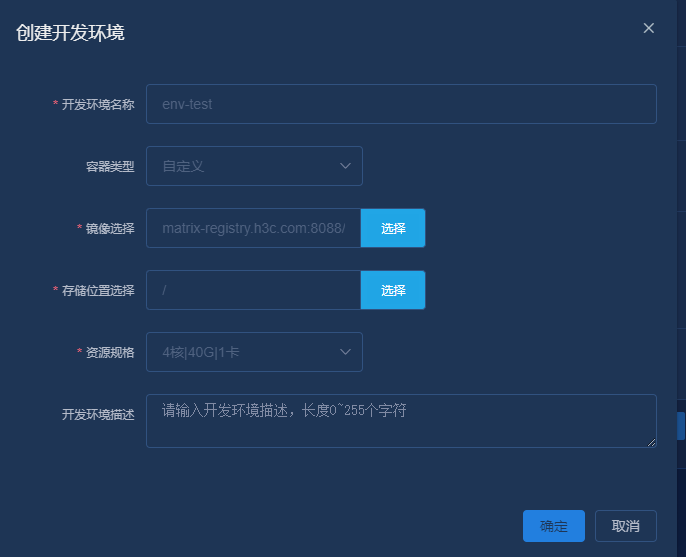
\includegraphics[width=0.7\textwidth]{figures/sigs-platform-dev-env-create.png}
	\caption{caption:sigs-platform-dev-env-create}
	\label{fig:sigs-platform-dev-env-create}
\end{figure}

\begin{figure}[htbp]
	\centering
	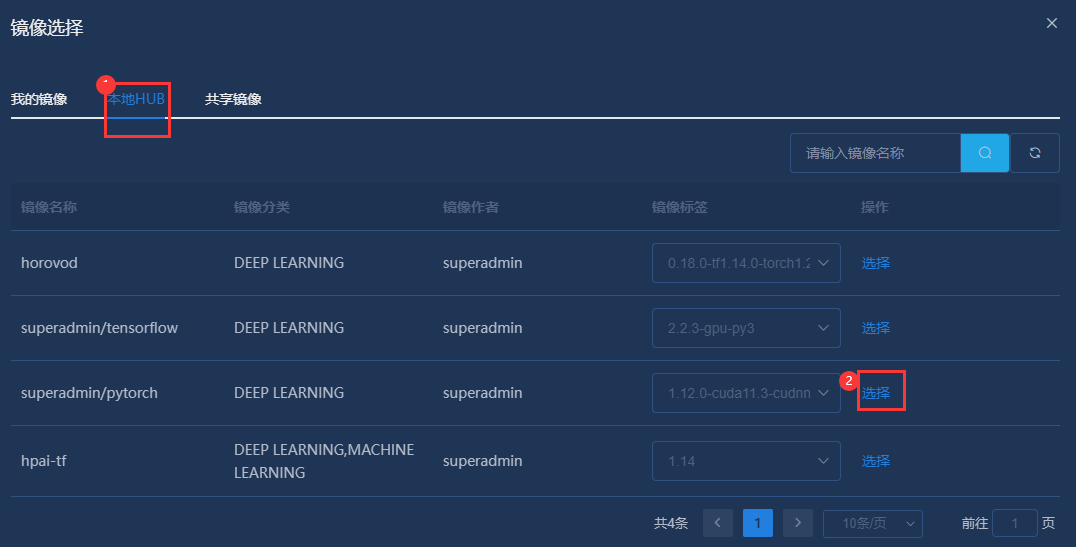
\includegraphics[width=0.7\textwidth]{figures/sigs-platform-dev-env-image-selection.png}
	\caption{caption:sigs-platform-dev-env-image-selection}
	\label{fig:sigs-platform-dev-env-image-selection}
\end{figure}

创建时指定的储存路径会挂载到环境的\graylstinline{/private}目录下。

\subsection{安装其他软件或包}

新建完成后,点击启动,等待镜像状态变为运行中,访问方式一栏会出现SSH、远程桌面和VNC三种连接方式,操作一栏的打开按钮也会有灰变蓝。

当我们需要使用镜像中尚未安装的工具或包时,可以通过访问方式提供的三种方式安装,譬如,在本地使用ssh连接服务器后,运行\graylstinline{conda install matplotlib}或\graylstinline{apt install git}等;也可通过点击打开按钮,在弹出页面中进入终端并安装,见图\ref{fig:sigs-platform-env-install-packages-via-web}。

\begin{figure}[htbp]
	\centering
	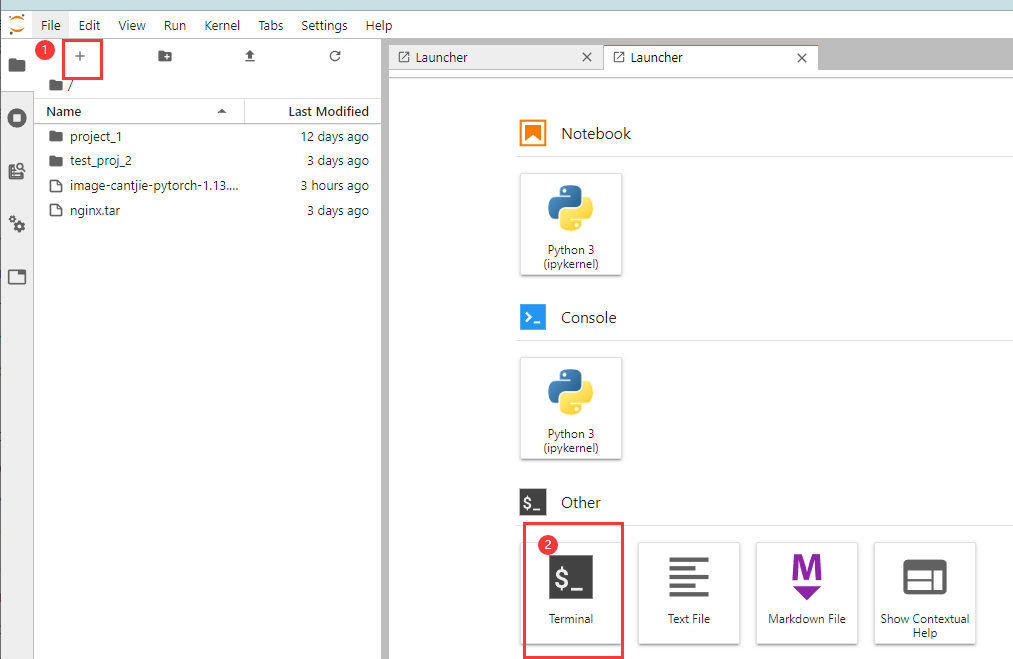
\includegraphics[width=0.7\textwidth]{figures/sigs-platform-env-install-packages-via-web.png}
	\caption{caption:sigs-platform-env-install-packages-via-web}
	\label{fig:sigs-platform-env-install-packages-via-web}
\end{figure}


\subsection{创建镜像环境}

\textcolor{red}{\emph{注意,截止本指导书书发布时,由于平台缺乏技术文档,个人制作的镜像可能无法让容器正常启动。该小节仍有待完善。}}

\textcolor{red}{\emph{注意,该平台为x86架构,arm平台上创建的镜像无法运行在该平台}}

镜像创建方法可参考\S\ref{subsec:container-to-image}。


在本地创建镜像后,使用\graylstinline{docker save -o filename.tar imagename:tag}\footnote{注意,此处不可使用sha256格式的imageID代替<imagename>:<tag>的格式,不然平台可能无法正确处理该镜像}命令导出镜像文件,然后上传至文件管理->我的文件栏目下(图\ref{fig:sigs-platform-upload-file})。然后在镜像服务->我的镜像中创建镜像(图\ref{fig:sigs-platform-create-custom-image})。

\begin{figure}[htbp]
	\centering
	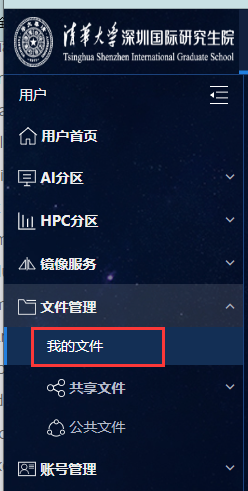
\includegraphics[width=0.3\textwidth]{figures/sigs-platform-upload-file.png}
	\caption{caption:sigs-platform-upload-file}
	\label{fig:sigs-platform-upload-file}
\end{figure}


\begin{figure}[htbp]
	\centering
	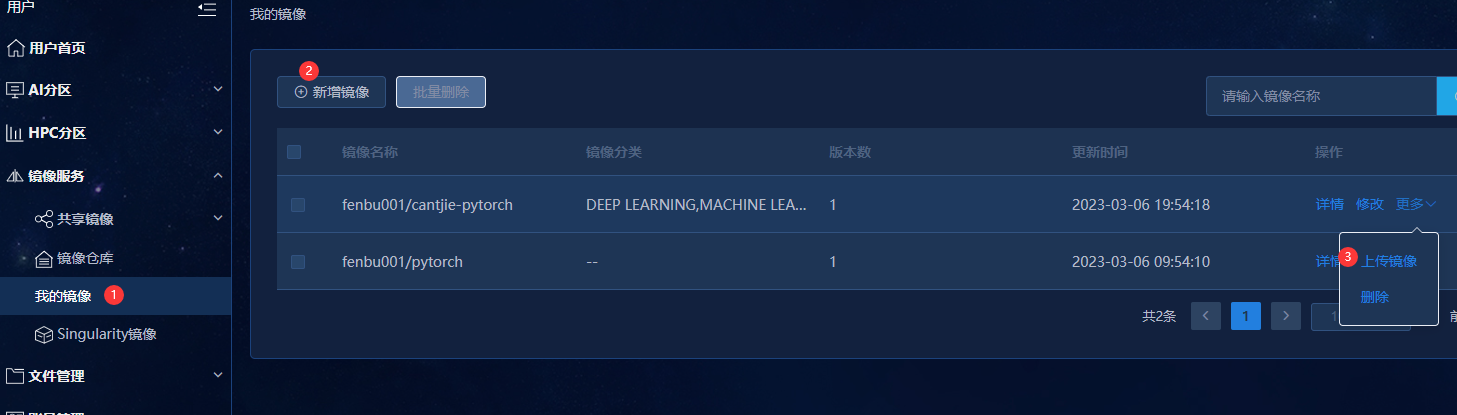
\includegraphics[width=1\textwidth]{figures/sigs-platform-create-custom-image.png}
	\caption{caption:sigs-platform-create-custom-image}
	\label{fig:sigs-platform-create-custom-image}
\end{figure}

\chapter{实验一:梯度下降单机优化}\label{chapter:task1}

\section{实验内容与要点介绍}

\subsection{实验内容与要求}

\subsubsection{实验内容}
\begin{itemize}
    \item 了解优化器的作用与构建方式(以PyTorch为例)
    \item 构建一阶确定性、一阶随机性优化算法,实现GD、SGD、Adam优化算法
    \item 分析确定性优化算法与随机性优化算法实验结果
\end{itemize}

\subsubsection{实验要求}
\begin{itemize}
    \item 在MNIST数据集上完成图像分类任务
    \item 实现GD、SGD、ADAM三种基于梯度的优化方法, 写出三个优化器类
    \item 绘制三种优化方法下的loss函数变化图像,通过loss图像及其他实验结果,分析三种优化方法的特点
\end{itemize}

\subsection{PyTorch优化器}

\subsubsection{优化器是干什么用的}

下面展示了一段简单的网络训练过程的代码,我们通过这段代码来理解PyTorch中优化器所发挥的作用。

\begin{lstlisting}
def train_loop(dataloader, model, loss_fn, optimizer):
    size = len(dataloader.dataset)
    for batch, (X, y) in enumerate(dataloader):
        # Compute prediction and loss
        pred = model(X)
        loss = loss_fn(pred, y)
        
        # Backpropagation
        optimizer.zero_grad()
        loss.backward()
        optimizer.step()
\end{lstlisting}
    
在这段代码中\graylstinline{model}为神经网络模型,通过\graylstinline{model(X)}调用了\graylstinline{model}中的\graylstinline{forward}方法,即进行正向传播,获得神经网络输出(第5行)。然后通过损失函数\graylstinline{loss_fn}计算神经网络输出\graylstinline{pred}与数据真实值或标签\graylstinline{y}的差距得到损失值\graylstinline{loss}(第6行)。
得到损失值后,通过反向传播(第10行),网络\graylstinline{model}中的各个参数对应的梯度将会得到更新,得到各个参数的梯度后,优化器\graylstinline{optimizer}便可以根据既定的优化算法来更新参数(第11行)。需要注意的是,神经网络的梯度参数并不是储存最近一次反向传播(即调用\graylstinline{loss.backward()})的结果,而是会将反向传播得到的梯度与当前储存的值相加。因此,我们需要第9行\graylstinline{optimizer.zero_grad()}来将神经网络\graylstinline{model}中储存的梯度值置为0。

如果你是第一次看到类似代码,你可能还会疑惑上述代码中优化器\graylstinline{optimizer}和\graylstinline{model}似乎并没有建立联系,那为什么优化器能处理\graylstinline{model}中的参数呢?这是因为在这个函数之外,\graylstinline{model}中的参数\graylstinline{model.parameters()}早就被喂给\graylstinline{optimizer}了:
\begin{lstlisting}
    optimizer = torch.optim.SGD(model.parameters(), lr=learning_rate)
\end{lstlisting}

\subsubsection{如何在优化器中实现自己的算法}

从上面的例子中可以看到,除了构建函数外,一个最简单的优化器只需要实现\graylstinline{zero_grad}和\graylstinline{step}方法即可。此处需要注意的有这几点:
\begin{itemize}
    \item 当我们手动更改\graphicspath{model}中参数或梯度的值时候,需要将其从计算图中分离。即在\graylstinline{zero_grad}方法中,应包含\graylstinline{param.grad.detach_()}。
    \item 使用Adam算法时,由于还需要上一步优化得到的状态,因此可在初始化函数中构建一个字典用来储存状态。
\end{itemize}

\subsection{MindSpore优化器}

除了使用Pytorch,我们还鼓励同学们使用MindSpore来完成实验。

在MindSpore中,可以通过继承\graylstinline{mindspore.nn.optim.optimizer.Optimizer}类来自定义自己的优化器。在Pytorch中,我们需要实现构造函数和\graylstinline{step()}函数,类似的,在MindSpore中,我们需要实现构造函数和\graylstinline{construct()}函数,\graylstinline{construct()}函数与\graylstinline{step()}函数作用类似。

在构造函数中,我们将神经网络参数、学习速率、衰减速率等变量存入实例。而与Pytorch的\graylstinline{step()}函数不同的是,\graylstinline{construct()}函数需要\graylstinline{gradients}参数作为输入。并且在计算完新的神经网络参数值后,需要使用\graylstinline{mindspore.ops.assign(old_param, new_param)}函数将新的参数值赋予神经网络。

一个简单的优化器实现如下:
\begin{lstlisting}
    from mindspore.nn.optim.optimizer import Optimizer
    from mindspore import ops

    class GdOptimizer(Optimizer):
        def __init__(self, params, lr=0.001):
            super(GdOptimizer, self).__init__(lr, params)

        
        def construct(self, gradients):
            success = None
            for param, grad in zip(self.parameters, gradients):
                update = param - self.learning_rate * grad
                success = ops.assign(param, update)
            return success
\end{lstlisting}

更多资料还可以参考mindspore官方文档:\url{https://mindspore.cn/tutorials/zh-CN/r2.0.0-alpha/advanced/modules/optimizer.html?highlight=%E8%87%AA%E5%AE%9A%E4%B9%89%E4%BC%98%E5%8C%96%E5%99%A8}

\subsection{几种算法回顾}

梯度下降 Gradient Descent:
\begin{align} 
w_{t+1} = w_t - \eta \nabla f(w_t)
\end{align}
随机梯度下降 Stochastic gradient descent:
\begin{align} 
w_{t+1} = w_t - \eta \nabla f_i(w_t)
\end{align}
Adam:
\begin{align} % amsmath package
    m_{t+1} & = \beta_1 m_t + (1-\beta_1) \nabla f(w_t)   \\
    g_{t+1} & = \beta_2 g_t + (1-\beta_2) (\nabla f(w_t))^2
\end{align}


\section{使用VSCode与本地环境调试运行}\label{sec:task1-local-debug}

如果你已经完成了本地环境配置(\S\ref{sec:local-env}),那就可以打开VSCode进行下面的操作了:

\begin{enumerate}
    \item 安装Python插件,如图\ref{fig:task1-vscode-extension-install-python}所示。
        \begin{figure}[htbp]
            \centering
            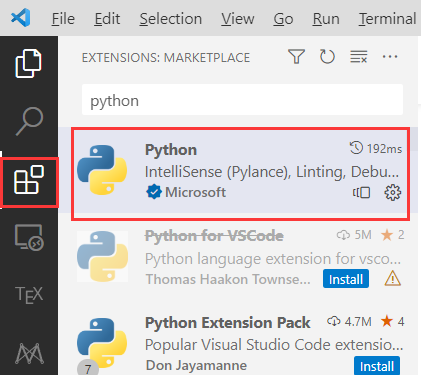
\includegraphics[width=0.7\textwidth]{figures/task1-vscode-extension-install-python.png}
            \caption{caption:task1-vscode-extension-install-python}
            \label{fig:task1-vscode-extension-install-python}
        \end{figure}
    \item 选择Python解释器,按下\graylstinline{F1}或\graylstinline{Ctrl}+\graylstinline{Shift}+\graylstinline{P},输入 "select interpreter"并选择 “Python: Select Interpreter”项(图\ref{fig:task1-vscode-local-select-interpreter})。然后选择:select at work space level。最后选择你在\S\ref{subsec:local-env-create}一孝节中创建的环境对应的解释器(图\ref{fig:task1-vscode-local-select-my-env}中为助教自己创建的distributedml环境)。
        \begin{figure}[htbp]
            \centering
            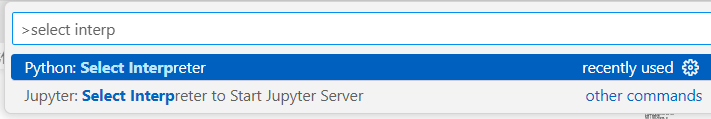
\includegraphics[width=0.7\textwidth]{figures/task1-vscode-local-select-interpreter.png}
            \caption{caption:task1-vscode-local-select-interpreter}
            \label{fig:task1-vscode-local-select-interpreter}
        \end{figure}
        \begin{figure}[htbp]
            \centering
            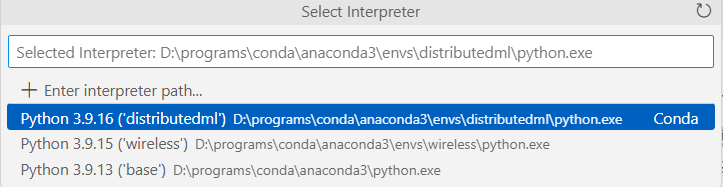
\includegraphics[width=0.7\textwidth]{figures/task1-vscode-local-select-my-env.png}
            \caption{caption:task1-vscode-local-select-my-env}
            \label{fig:task1-vscode-local-select-my-env}
        \end{figure}
    \item 最后,打开自己的.py文件,可以在编辑器右上角看到一个播放形状的三角,点击它或在下拉列表中选择运行或调试,即可开始运行或调试啦。
    \begin{figure}[htbp]
        \centering
        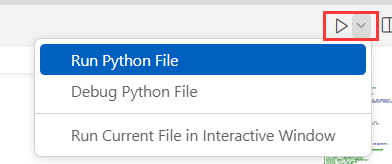
\includegraphics[width=0.5\textwidth]{figures/task1-vscode-local-run-or-debug.png}
        \caption{caption:task1-vscode-local-run-or-debug}
        \label{fig:task1-vscode-local-run-or-debug}
    \end{figure}
\end{enumerate}


\section{使用VSCode与本地容器调试运行}\label{sec:vscode-and-docker-container}

\subsection{启动容器并挂载本地文件夹}\label{subsec:docker-run-and-mount-volume}

在\S\ref{subsec:container-to-image}一小节中,我们创建了自己的镜像,现在,我们需要先启动这个镜像(对于助教而言是\graylstinline{cantjie/pytorch:1.13.1})。但是,目前镜像里面可没有我们写好的代码,而且,就算我们在镜像里面写好代码,该怎么拿出来交作业呢?

为了解决这个问题,我们就需要将本地的目录挂载到容器上,在启动容器时,我们使用\graylstinline{-v <host-dir>:<container-dir>}参数,参考下面命令执行:
\begin{lstlisting}
    $ docker run -it --gpus all -v $pwd/relative/path/to/code:/workspace cantjie/pytorch:1.13.1
\end{lstlisting}

现在进入容器后,我们可以看到,如图\ref{fig:task1-docker-run-with-mount}所示,本地的代码已经被挂载到了\graylstinline{\workspace}文件夹下。
\begin{figure}[htbp]
	\centering
	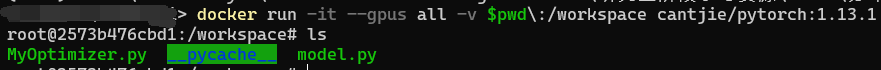
\includegraphics[width=0.9\textwidth]{figures/task1-docker-run-with-mount.png}
	\caption{caption:task1-docker-run-with-mount}
	\label{fig:task1-docker-run-with-mount}
\end{figure}

\subsection{在VSCode中使用容器}

首先安装Dev Container插件,然后按下\graylstinline{Ctrl}+\graylstinline{Shift}+\graylstinline{P},并找到Attatch to Running Container命令,如图\ref{fig:task1-vscode-attach-to-container-quick-search}。
\begin{figure}[htbp]
	\centering
	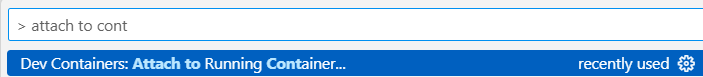
\includegraphics[width=0.7\textwidth]{figures/task1-vscode-attach-to-container-quick-search.png}
	\caption{caption:task1-vscode-attach-to-container-quick-search}
	\label{fig:task1-vscode-attach-to-container-quick-search}
\end{figure}

接下来会弹出一个新窗口,在这个新窗口中,就像在本地环境下调试运行一样在容器里调试运行即可。余下的步骤基本参考上一小节\S\ref{sec:task1-local-debug}中的操作即可。即
\begin{itemize}
    \item 在VSCode侧边栏Explorer栏目中打开\graylstinline{/workspace}目录。
    \item 在VSCode安装Python插件。
    \item 选择编译器为\graylstinline{/opt/conda/bin/python}
\end{itemize}

\section{使用VSCode与远程服务器调试运行}

% 深研院平台和华为云平台的远程服务器使用方法类似,此处以学校的环境为例。
\subsection{使用深研院计算资源}\label{subsec:task1-vscode-using-sigs-resources}
在学校的计算平台创建了开发环境后,平台会提供ssh链接地址以及用户名和密码,我们使用该信息链接远程环境。

首先在VSCode中安装Remote SSH插件,然后按下\graylstinline{Ctrl}+\graylstinline{Shift}+\graylstinline{P},搜索Remote-SSH: Open SSH Configuration File命令(图\ref{fig:task1-open-ssh-config-file})。
\begin{figure}[htbp]
	\centering
	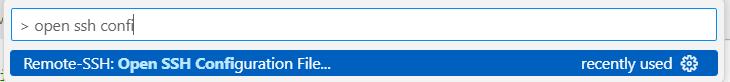
\includegraphics[width=0.7\textwidth]{figures/task1-open-ssh-config-file.png}
	\caption{caption:task1-open-ssh-config-file}
	\label{fig:task1-open-ssh-config-file}
\end{figure}

在下拉列表中选择 C:\textbackslash Users\textbackslash <username>\textbackslash .ssh.

\begin{figure}[htbp]
	\centering
	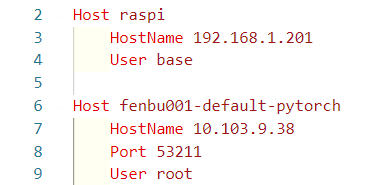
\includegraphics[width=0.6\textwidth]{figures/task1-ssh-config-file-demo.png}
	\caption{ssh config file demo。注意,图中示例包含两个主机。}
	\label{fig:task1-ssh-config-file-demo}
\end{figure}

在打开的.ssh文件中, 按照图\ref*{fig:task1-ssh-config-file-demo}给出的格式,添加一个主机。其中Host对应昵称,HostName为远程主机IP。

\begin{figure}[htbp]
	\centering
	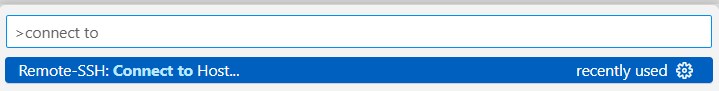
\includegraphics[width=0.7\textwidth]{figures/task1-vscode-connect-to-host-quick-search.png}
	\caption{caption:task1-vscode-connect-to-host-quick-search}
	\label{fig:task1-vscode-connect-to-host-quick-search}
\end{figure}

最后,\graylstinline{Ctrl}+\graylstinline{Shift}+\graylstinline{P}并搜索Remote-SSH: Connect to Host命令,并在后续选择刚刚创建的主机信息。

\begin{figure}[htbp]
	\centering
	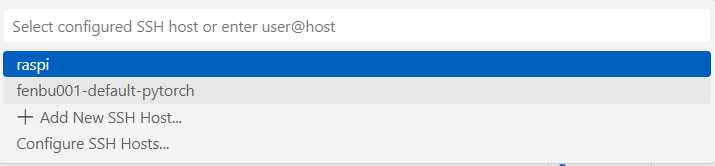
\includegraphics[width=0.7\textwidth]{figures/taks1-vscode-connect-to-certain-host-quick-search.png}
	\caption{caption:taks1-vscode-connect-to-certain-host-quick-search}
	\label{fig:taks1-vscode-connect-to-certain-host-quick-search}
\end{figure}

在弹出的窗口等待连接,并输入密码。余下的步骤又和上一小节\S\ref{sec:vscode-and-docker-container}一样了:打开文件夹、安装Python扩展、指定解释器。此处不再赘述。

\subsection{使用华为云计算资源}

\subsubsection{手动配置}

同使用深研院计算资源\S\ref{subsec:task1-vscode-using-sigs-resources}一样,我们也通过编辑C:\textbackslash Users\textbackslash <username>\textbackslash .ssh中的config文件,来配置ssh链接。在配置前,首先进入华为云的开发环境实例中查看实例的ssh地址,如图\ref{fig:task1-huawei-modelarts-ssh-address}所示,该实例对应的用户名、地址和端口分别为\graylstinline{ma-user}、\graylstinline{dev-modelarts-cnnorth4.huaweicloud.com}、\graylstinline{30194}。

\begin{figure}[htbp]
	\centering
	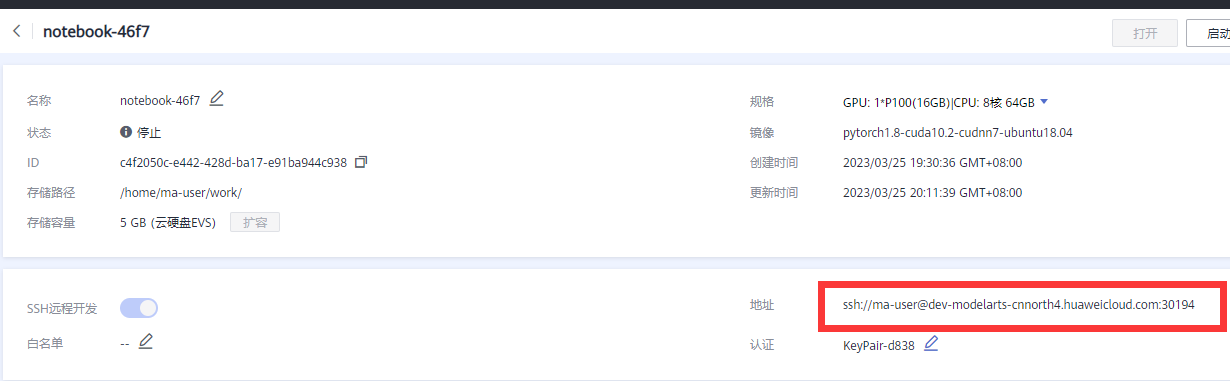
\includegraphics[width=0.9\textwidth]{figures/task1-huawei-modelarts-ssh-address.png}
	\caption{caption:task1-huawei-modelarts-ssh-address}
	\label{fig:task1-huawei-modelarts-ssh-address}
\end{figure}


打开config文件,在原来的基础上加入如图\ref{fig:task1-huawei-modelarts-ssh-config-demo}所示内容。注意根据你的实例和秘钥对修改其中HostName、Port、User、IdentityFile字段。

\begin{figure}[htbp]
	\centering
	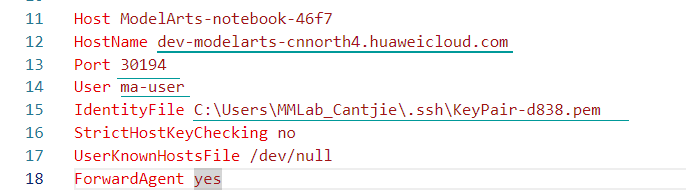
\includegraphics[width=0.8\textwidth]{figures/task1-huawei-modelarts-ssh-config-demo.png}
	\caption{caption:task1-huawei-modelarts-ssh-config-demo}
	\label{fig:task1-huawei-modelarts-ssh-config-demo}
\end{figure}

然后又和上一节一样了,用Remote-SSH插件的Connect to Host命令接入该实例即可。

\subsubsection{使用ModelArts插件自动配置}

聪明的你可能已经发现不同于深研院的平台,华为ModelArts平台中,开发环境实例最右侧操作的更多选项里有一个VS Code接入选项,图\ref{fig:task1-huawei-modelarts-vscode-auto-connect}。如果我们已经安装了VS Code的Remote-SSH插件,我们直接点击“VS Code接入”就可以开始远程开发了。
\begin{figure}[htbp]
	\centering
	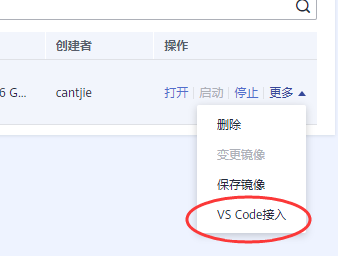
\includegraphics[width=0.4\textwidth]{figures/task1-huawei-modelarts-vscode-auto-connect.png}
	\caption{caption:task1-huawei-modelarts-vscode-auto-connect}
	\label{fig:task1-huawei-modelarts-vscode-auto-connect}
\end{figure}

第一次点击的时候,可能会提示你没有安装一个ModelArts-HuaweiCloud插件,如图\ref{fig:task1-huawei-modelarts-vscode-auto-connect-extension-error},我们点击Install and Open即可。




\begin{figure}[htbp]
	\centering
	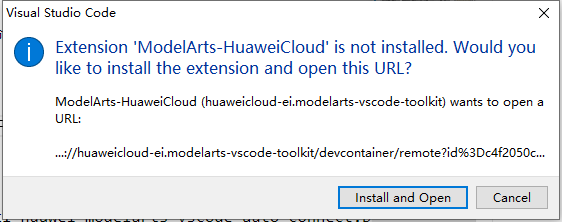
\includegraphics[width=0.6\textwidth]{figures/task1-huawei-modelarts-vscode-auto-connect-extension-error.png}
	\caption{caption:task1-huawei-modelarts-vscode-auto-connect-extension-error}
	\label{fig:task1-huawei-modelarts-vscode-auto-connect-extension-error}
\end{figure}

这时如果你打开C:\textbackslash Users\textbackslash <username>\textbackslash .ssh\textbackslash config文件,你会发现刚刚安装的插件的作用其实就是帮你自动写入图\ref{fig:task1-huawei-modelarts-ssh-config-demo}中的内容。


\subsection{使用密钥对登录远程服务器(可选)}

在使用深研院计算资源和docker容器的时候,你可能已经发现,每次登录都要输入密码,有点麻烦。我们现在可以使用密钥对来实现免密登录远程服务器或容器。

具体而言,在本地(以助教的windows为例),打开终端,使用\graylstinline{ssh-keygen}命令,生成一对秘钥对:
\begin{lstlisting}
    ssh-keygen -t ed25519
\end{lstlisting}
然后在提示下按下三次回车,当然你也可以选择自定义这些内容,不过一般使用默认的设置和空的passphrase就可以了。


我们按照第一次按回车时提示的目录,找到这对密钥对,对于windows,一般是在:
C:\textbackslash Users \textbackslash <username>\textbackslash .ssh目录下的\graylstinline{id_ed25519}私钥文件和\graylstinline{id_ed25519.pub}的公钥文件。

接下来我们需要将公钥文件发送给服务器或容器。如果你的终端可以运行\graylstinline{ssh-copy-id}命令,那么你只需要在终端运行下面的命令即可将公钥发送。
\begin{lstlisting}
    ssh-copy-id user@serverip
\end{lstlisting}

然而,如果你的终端找不到\graylstinline{ssh-copy-id}命令,那么发送过程会稍微麻烦一些:手动将公钥内容写入服务器的\graylstinline{\~/.ssh/authorized_keys}文件中:
\begin{lstlisting}
    # first ssh into the server or container
    # copy the content of your <id_ed25519.pub> into <authorized_keys>
    vi \~/.ssh/authorized_keys
    
    # give the <authorized_keys> propoer permissions
    chmod 600 ~/.ssh/authorized_keys    
\end{lstlisting}
这样就完成公钥的发送了。之后你从终端ssh到服务器,就不再需要密码了。


\subsubsection{可能的问题:权限错误}

如果你在ssh时遇到了权限错误的提示,那很可能是你的本地的私钥的权限出问题了。找你的私钥文件,右键查看属性,在<安全>标签页点击编辑。如果你发现<组或用户名>栏目中有多个项目,如图\ref{fig:task1-ssh-private-key-permission-in-windows}所示(其中马赛克挡住的应该是你目前登录的用户),那么你需要将除了你自己之外的其他用户都删掉,变成图\ref{fig:task1-ssh-private-key-right-permission-in-windows}所示的那样。

\begin{figure}[htbp]
	\centering
	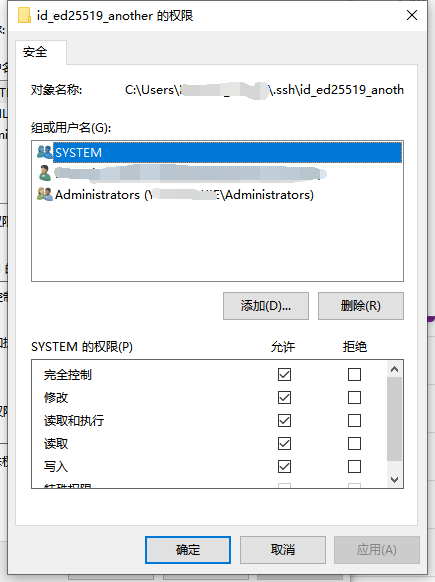
\includegraphics[width=0.7\textwidth]{figures/task1-ssh-private-key-permission-in-windows.png}
	\caption{caption:task1-ssh-private-key-permission-in-windows}
	\label{fig:task1-ssh-private-key-permission-in-windows}
\end{figure}


\begin{figure}[htbp]
	\centering
	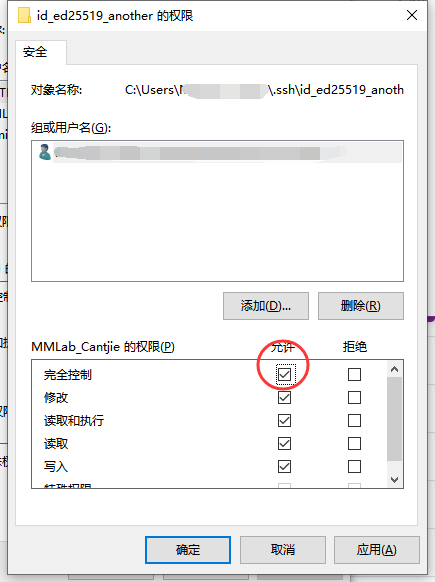
\includegraphics[width=0.7\textwidth]{figures/task1-ssh-private-key-right-permission-in-windows.png}
	\caption{caption:task1-ssh-private-key-right-permission-in-windows}
	\label{fig:task1-ssh-private-key-right-permission-in-windows}
\end{figure}
\chapter{实验二:通信模型与参数聚合}

\section{实验内容与要点介绍}

\subsection{实验内容与要求}

\subsubsection{实验内容}
\begin{itemize}
    % \item 了解并掌握分布式算法中的集体通信和参数聚合策略,了解并掌握集体通信中常用的消息传递接口(Reduce, AllReduce, Gather, AllGather, Scatter, etc.)
    % \item 实现模型参数或模型参数梯度的聚合,尝试使用不同聚合方式(Sum, Mean, etc.)对模型的参数和梯度进行聚合,并分析不同聚合策略对模型性能的影响。    
    \item 了解集体通信中的常用消息传递接口(Reduce,AllReduce,Gather,AllGather,Scatter 等);
    \item 基于集体通信进行模型参数(梯度)聚合更新,尝试使用不同聚合方式(Sum, Mean, etc.)对模型的参数和梯度进行聚合;
    \item 分析不同聚合策略对模型性能的影响。
\end{itemize}

\subsubsection{实验要求}
\begin{itemize}
    \item 实现集体通信下的参数(梯度)聚合,基于至少2种集体通信原语实现梯度平均的聚合方法,并比较它们的通信时间开销,分析不同聚合策略对模型性能的影响
    \item 在框架下设置瓶颈节点,讨论瓶颈节点对集体通信的影响。
\end{itemize}

\subsection{多节点通信}

在本次实验中,我们采用PyTorch中的\graylstinline{torch.distributed}模块(下面将简写为\graylstinline{dist})作为多节点通信的支持工具。

\subsubsection{初始化进程组}\label{subsubsec:task2-init-process-group}

多节点通信的第一步,是初始化进程组。因此每个节点在训练之前,需要先调用\graylstinline{dist.init_process_group()}函数来初始化进程。这个函数会阻塞当前进程,并等待其他进程加入,阻塞持续至直到所有节点(进程)都加入了进来。

对于本次实验,我们需要关注这个函数的三个输入:\graylstinline{backend},\graylstinline{world_size}和\graylstinline{rank}。
\begin{itemize}
    \item \graylstinline{backend}指定通信后端,即实现多节点通信的底层的通信协议,对于本次实验,当在Linux环境下且使用GPU时,一般选择nccl,其他情况下,一般使用gloo即可(每种后端支持的设备类型和功能有所不同,更多内容可阅读官方文档\url{https://pytorch.org/docs/stable/distributed.html#backends})。
    \item \graylstinline{world_size}为进程总数。
    \item \graylstinline{rank}指定当前进程的优先级。启动多节点时,需要为每个进程指定rank,一般为每个进程赋值为0到进程总数-1中的整数。
\end{itemize}

但是光有这三个参数还不足以让多节点(进程)之间可以发现彼此,其实还需要告诉节点主进程的通信地址和端口。这里我们采用设置环境变量的方式告诉节点们如何找到\graylstinline{rank=0}的主节点。下面这段代码展示了\graylstinline{rank=0}的节点的初始化方式。
\begin{lstlisting}
    import torch.distributed as dist

    # change it to the corresponding ip addr
    os.environ['MASTER_ADDR'] = 'localhost'
    os.environ['MASTER_PORT'] = 12355
    
    # initialize the process group
    dist.init_process_group(backend="nccl", rank=0, world_size=2)
\end{lstlisting}

\subsubsection{广播模型参数}

完成进程组初始化后,在神经网络模型训练开始前,需要确保所有节点上的模型是一样的,因此需要将主节点上的模型的参数广播给其他所有节点。我们使用\graylstinline{dist.broadcast()}函数来同步所有节点的参数。

下面这段代码展示了广播过程,\graylstinline{dist.broadcast()}需要两个参数:
\begin{itemize}
    \item \graylstinline{tensor},为需要广播或接收的数据。当广播源为当前进程时,\graylstinline{tensor}将被发送给其他节点,当广播源不是当前进程时,\graylstinline{tensor}将被赋为接收到的数据。
    \item \graylstinline{src},为广播源的rank。
\end{itemize}

\begin{lstlisting}
    if get_world_size() > 1:
        for param in model.parameters():
            dist.broadcast(tensor=param.data,src=0)
\end{lstlisting}

\subsubsection{参数聚合}

神经网络模型训练过程中,就要实现参数聚合了。该部分请同学们自行完成。

\subsection{记录GPU上任务的运行时间}

利用\graylstinline{torch.cuda.Event.elapsed_time()}记录,示例代码如下:
\begin{lstlisting}
    start_evt = torch.cuda.Event(enable_timing=True)
    end_evt = torch.cuda.Event(enable_timing=True)
    start_evt.record()
    # the time between start_evt and end_evt will be caculated
    end_evt.record()
    torch.cuda.synchronize()
    whole_time = start_evt.elapsed_time(end_evt)
\end{lstlisting}

\section{使用进程模拟多节点}

为了模拟多节点通信,我们可以在同一台机器上使用不同进程或容器来实现。本节介绍多节点模拟的方法。通过进程模拟的方法在本地、在本地容器中、在华为云、在学校的计算平台都是通用的。

\subsection{手动运行多进程}
启动两个终端,分别指定不同的rank即可。例如:
\begin{lstlisting}[language=bash]
    # first process:
    $ python model.py --n_devices=2 --rank=0
    # second process:
    $ python model.py --n_devices=2 --rank=1
\end{lstlisting}

\subsection{使用torch.multiprocessing自动创建多进程}

通过\graylstinline{torch.multiprocessing}中的\graylstinline{spawn()}函数即可让该函数自动帮我们创建多个进程,其中,我们需要关注该函数的三个参数:
\begin{itemize}
    \item \graylstinline{fn}为函数名,将作为生成的进程的入口。
    \item \graylstinline{args}为tuple元组类型。每个进程将通过 \graylstinline{fn(i, *args)}的方式调用\graphicspath{fn},其中\graylstinline{i}即为所生成进程的rank,从0开始逐次递增1。
    \item \graylstinline{nprocs}为生成的进程总数,即前文所指的\graylstinline{worldsize}或\graylstinline{n_devices}。
\end{itemize}

下面一段代码简要说明了\graylstinline{spawn()}函数的使用方法。详情可参考\graylstinline{model-mp.py}。
\begin{lstlisting}
import torch.multiprocessing as mp
def main(rank, args):
    pass
if __name__ == "__main__":
    args = parse_args()
    mp.spawn(main, (args,), nprocs=args.n_devices)
\end{lstlisting}

\section{使用容器模拟多节点}

“容器就类似于虚拟机了,那通过容器模拟多节点岂不是更真实?”不知道有多少同学也和助教一样这样以为过。那我们就来尝试一下看起来更高端的容器模拟多节点吧。

注意,由于我们只在本地安装了docker并自定义了镜像(\S\ref{subsec:container-to-image}),所以下面的内容针对的是在本地使用容器模拟的过程。当然只要你掌握了方法,在远程的平台上也是一样使用的。

乍一看上去很复杂,多个容器之间的通信怎么处理呢?其实完全不用担心,我们只要使用docker compose就可以了,它会帮我们自动配置好同一组容器下的网络。

\subsection{Docker compose介绍}

如果你也在windows下,并且安装了docker desktop,那么docker compose已经是自带得了,不需要额外安装了。docker compose就是通过使用一个模板文件(yaml格式)来定义一组的相关联的应用容器的程序。我们首先来看一下这个所谓的模板文件是什么样的叭。

我们以助教发给大家的\graylstinline{docker-compose.yml}为例,我们取其中的一部分先简单分析一下这个文件的内容。
\begin{lstlisting}
services:
    node01:           
        # container_name: node01
        image: cantjie/pytorch:1.13.1
        volumes:
          - .:/workspace      # <host(local) dir (should start with . or /)>:<dir in container>
        command:              # python /workspace/model.py --n_devices=1 --rank=0 --gpu=0
          - python
          - -u
          - /workspace/model.py 
          - --n_devices=2
          - --rank=0
          - --gpu=0
          - --master_addr=localhost
          - --master_port=12378
        deploy:              # make GPU accessible in container
          resources:
            reservations:
              devices:
                - driver: nvidia
                  count: 1
                  capabilities: [gpu]
\end{lstlisting}

文件中定义了两个\graylstinline{services},每个\graylstinline{service}就对应了一个容器,对于每个容器的配置,以\graylstinline{node01}为例,我们通过\graylstinline{image}指定了镜像,通过\graylstinline{volumes}指定了文件挂载路径(参考\S\ref{subsec:docker-run-and-mount-volume}),通过\graylstinline{command}指定了容器启动后需要执行的命令,下面这个写法实际上是告诉容器执行这条语句:
\begin{lstlisting}[language=bash]
    $ python -u /workspace/model.py --n_devices=2 --rank=0 --gpu=0 \
        --master_addr=localhost --master_port=12378
\end{lstlisting}
其中\graylstinline{-u}表示将Python中\graylstinline{print}命令的输出以unbuffer的方式输出,这是docker容器的一个特性,如果不加\graylstinline{-u},我们只能在训练完成、代码跑完之后才能看到程序输出的结果啦。

最后的\graylstinline{deploy}则是让容器能够使用宿主机的GPU(\graylstinline{deploy}这一段是网上复制来哒,细问我也不懂啦)。

至于\graylstinline{node02},除了\graylstinline{rank}外,只有\graylstinline{master_addr}与\graylstinline{node01}不同,对于\graylstinline{node01}来说,master就是自己了,而对于\graylstinline{node02}来说,master当然是\graylstinline{node01}了。

你可能要问,那为什么这里不是写master的ip,而是写“node01”就行了呢?这就是Docker compose的方便之处了,他会自动修改容器内的hosts,也就是“node01”就是\graylstinline{node01}这个节点的“域名”了。

\subsection{通过Docker compose启动容器}

将这个文件和\graylstinline{model.py}放到同一个目录下,然后终端\graylstinline{cd}到这里,输入\graylstinline{docker compose up}就完成啦,我们就可以看到程序已经开始训练了!如图\ref{fig:task2-docker-compose-up}所示。


\begin{figure}[htbp]
	\centering
	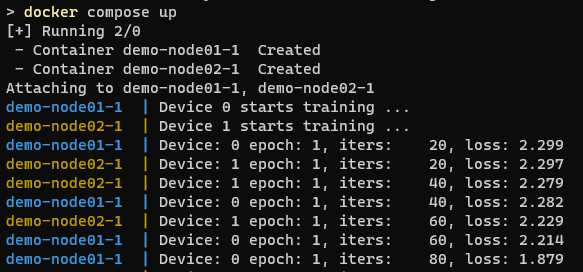
\includegraphics[width=0.7\textwidth]{figures/task2-docker-compose-up.png}
	\caption{caption:task2-docker-compose-up}
	\label{fig:task2-docker-compose-up}
\end{figure}

这里还需要注意的是,由于我们在yaml中,并没有使用\graylstinline{container_name}为容器指定名字,因此Docker生成容器的时候,会按照\graylstinline{<dir>-<service-name>-<number>}命名方式为我们的容器命名,如果你的\graylstinline{docker-compose.yml}处在一个中文名称的文件夹下,系统很可能会报错的。放到英文命名的文件夹下就好了。

\chapter{实验三:数据并行}

\section{实验内容}

\chapter{实验四:模型并行实验}

\section{实验内容}


% \chapter{Introduction}\label{introduction}

% \citet{anderson1985phonology} is a book that should now show up in the references.

% \begin{exe} \ex \label{staednacds} \begin{xlist}
% % \ex[] {*I don’t [go e\textturnr].}
% % \ex[] {I don’t [go ðe\textturnr]. }
% \end{xlist}
% \end{exe}


% \begin{exe} 
% \ex[] {Don't [it\textsuperscript{h}:\ae t].}
% \end{exe}



% \section {Discussion}

% Here's another example, see \ref{ex:example} for the example.

% \begin{exe}
% \ex\label{ex:example} Here's an \textbf{example}.
% \end{exe}

% \subsection{A subsection}
% Some text

% \begin{figure}[ht] %puts a figure either here or the top of the next page.
%     \centering
% %    \includegraphics[width=0.6\linewidth]{deleter-r-stats.png}
%     \caption{Caption}
%     \label{fig:mylabel}
% \end{figure}
 

% \subsection{Another subsection}

% \section{Conclusion}


    

\clearpage\singlespacing


%\phantomsection

% \bibliography{references/Bibliog}  %Name of your bibliography file, exported from Zotero.


\end{document}

